\chapter{Routine Use of {\LaTeX} }

Most documents contain forward references to \verb|\label|s.  So, often we
must latex the files twice.

\section{Document Structure}

The macro \verb|\chapter| is self-explantory.  These also introduce a
line in the table of contents (.toc) file.  The .toc file is generated
at the end of LaTeX processing.  So, to include a table of contents
properly at the beginning of the document, we must {\tt pdflatex} the
files twice.

The depth of sections that show up in the TOC is typically set in the
report style to 3.  You can change this, to say 9, by including the
line\\ {\tt \verb|\setcounter|\{secnumbookdepth\}\{9\}} in {\tt thesis.tex}.

\section{Lists}

LaTeX has three kinds of lists.  Description list is often better than
{\tt enumerate} which is better than {\tt itemize}.

\section{Figures}

Figures and tables float, often ending up at the top of a page, or
even at the end of the document.  To control this, learn the
\verb|!htb| options of the {\tt figure} environment.  
Figures should be no more than a single page; rework them if
they are not.

Each of the \TeX/ \LaTeX{} specific packages {\tt eepic}, {\tt
  pstricks}, {\tt graphicx}, and {\tt tikz} is capable of producing
intricate drawings, but the learning curve is steep.
You must explore the collection of figures at
\url{www.texample.net}.

\subsection{\LaTeX{} File Genreated by {\tt xfig}}

Figure \ref{trie} was interactively drawn using {\tt xfig} and then
exported as a .tex file from it.  Typcially, we \verb|\label| the
figures so we can reference it.  Look at the source \LaTeX{} file of
this chapter.

\begin{figure}[ht]\centering
\setlength{\unitlength}{3947sp}%
%
\begingroup\makeatletter\ifx\SetFigFont\undefined%
\gdef\SetFigFont#1#2#3#4#5{%
  \reset@font\fontsize{#1}{#2pt}%
  \fontfamily{#3}\fontseries{#4}\fontshape{#5}%
  \selectfont}%
\fi\endgroup%
\begin{picture}(5787,3030)(751,-3586)
\thinlines
\put(4726,-1486){\vector(-1, 0){2625}}
\put(5326,-1486){\vector(-1, 0){375}}
\put(1951,-1636){\vector( 3,-1){2475}}
\put(3826,-736){\vector( 4,-1){2700}}
\put(2776,-2611){\vector(-1, 0){1425}}
\put(4276,-2611){\vector(-1, 0){1200}}
\put(1276,-3511){\vector(-1, 0){225}}
\put(2551,-3511){\vector(-1, 0){300}}
\put(3076,-3511){\vector(-1, 0){300}}
\put(3676,-3511){\vector(-1, 0){225}}
\put(4426,-2761){\vector( 0,-1){675}}
\put(3001,-2761){\vector( 3,-2){900}}
\put(1201,-2761){\vector( 1,-3){225}}
\put(1726,-1561){\makebox(0,0)[lb]{\smash{\SetFigFont{12}{14.4}{\rmdefault}{\mddefault}{\updefault}a:16}}}
\put(4801,-1561){\makebox(0,0)[lb]{\smash{\SetFigFont{12}{14.4}{\rmdefault}{\mddefault}{\updefault}b}}}
\put(5401,-1561){\makebox(0,0)[lb]{\smash{\SetFigFont{12}{14.4}{\rmdefault}{\mddefault}{\updefault}c}}}
\put(5926,-1561){\makebox(0,0)[lb]{\smash{\SetFigFont{12}{14.4}{\rmdefault}{\mddefault}{\updefault}...}}}
\put(3601,-661){\makebox(0,0)[lb]{\smash{\SetFigFont{12}{14.4}{\rmdefault}{\mddefault}{\updefault}root}}}
\put(6526,-1561){\makebox(0,0)[lb]{\smash{\SetFigFont{12}{14.4}{\rmdefault}{\mddefault}{\updefault}z}}}
\put(1051,-2686){\makebox(0,0)[lb]{\smash{\SetFigFont{12}{14.4}{\rmdefault}{\mddefault}{\updefault}n:5}}}
\put(3751,-3586){\makebox(0,0)[lb]{\smash{\SetFigFont{12}{14.4}{\rmdefault}{\mddefault}{\updefault}t:0}}}
\put(2851,-2686){\makebox(0,0)[lb]{\smash{\SetFigFont{12}{14.4}{\rmdefault}{\mddefault}{\updefault}r:0}}}
\put(4351,-3586){\makebox(0,0)[lb]{\smash{\SetFigFont{12}{14.4}{\rmdefault}{\mddefault}{\updefault}e:1}}}
\put(2551,-3586){\makebox(0,0)[lb]{\smash{\SetFigFont{12}{14.4}{\rmdefault}{\mddefault}{\updefault}e:3}}}
\put(3151,-3586){\makebox(0,0)[lb]{\smash{\SetFigFont{12}{14.4}{\rmdefault}{\mddefault}{\updefault}m:1}}}
\put(751,-3586){\makebox(0,0)[lb]{\smash{\SetFigFont{12}{14.4}{\rmdefault}{\mddefault}{\updefault}d:2}}}
\put(1351,-3586){\makebox(0,0)[lb]{\smash{\SetFigFont{12}{14.4}{\rmdefault}{\mddefault}{\updefault}t:1}}}
\put(2026,-3586){\makebox(0,0)[lb]{\smash{\SetFigFont{12}{14.4}{\rmdefault}{\mddefault}{\updefault}c:1}}}
\put(4426,-2686){\makebox(0,0)[lb]{\smash{\SetFigFont{12}{14.4}{\rmdefault}{\mddefault}{\updefault}t:1}}}
\end{picture}

\caption{The figure above is drawn by {\tt Figures/trie.tex} using
  vectors built-in \LaTeX{}}\label{trie}
\end{figure}

You can include an eps or pdf file generated by any drawing tool.

\subsection{JPG and PNG Images}

\begin{table}[htb]
\begin{tabular}{lr}\hline
 \parbox{0.75\textwidth}
         {\TBD{} You can include a .jpg, .png, ...
  file using {\tt includegraphics} while scaling it.  Here we show
  the figure of {\tt Figures/gps-track-line.png}.
  A package named {\tt wrapfig} gives greater control.
}
&
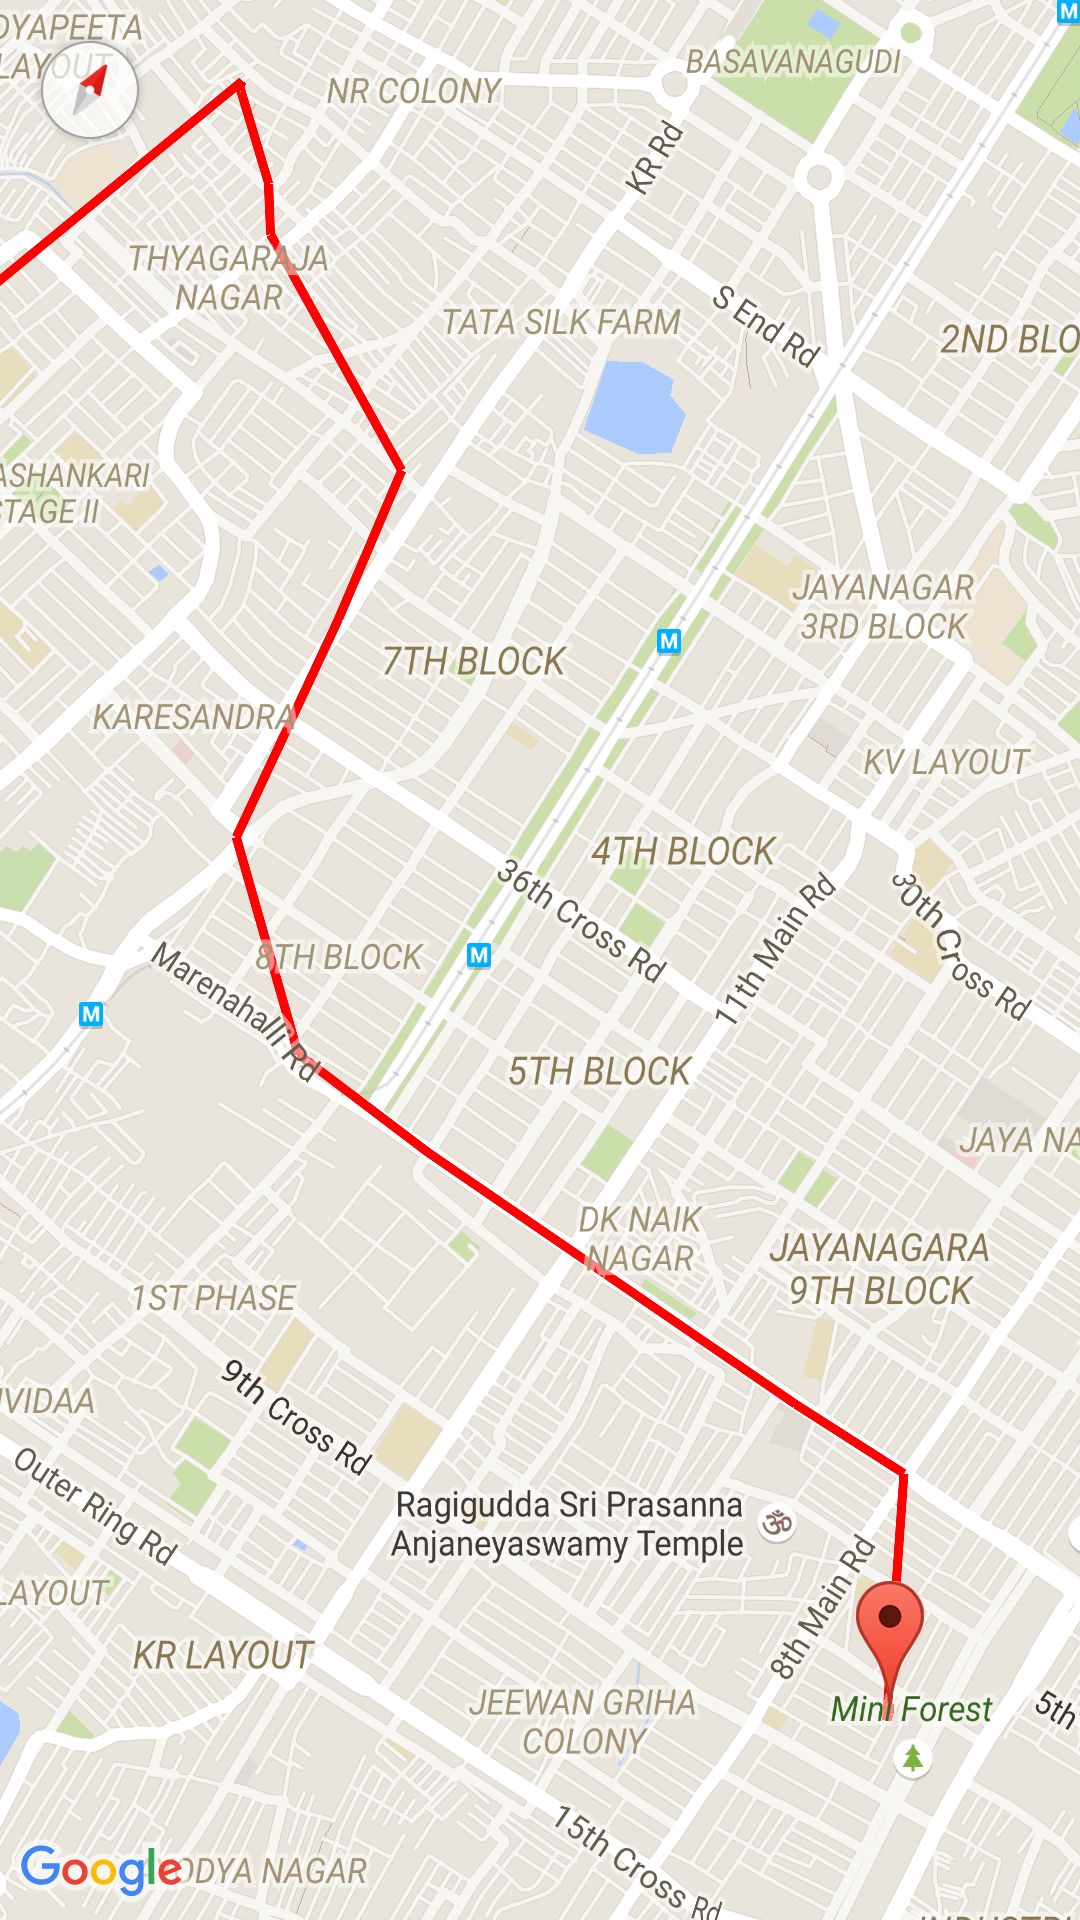
\includegraphics[scale=0.08]{Figures/gps-track-line.png}
\end{tabular}
\caption{This is a table beacuse we used the {\tt table} environment.}
\label{fig:gps-track-line.png}
\end{table}

The ``table'' \ref{fig:gps-track-line.png} is referenced here, and yet
it shows up at the top of the page.  This is known as floating, and we
permitted it by the {\tt htb} options.

\subsection{PDF}

\begin{minipage}{5.0cm}
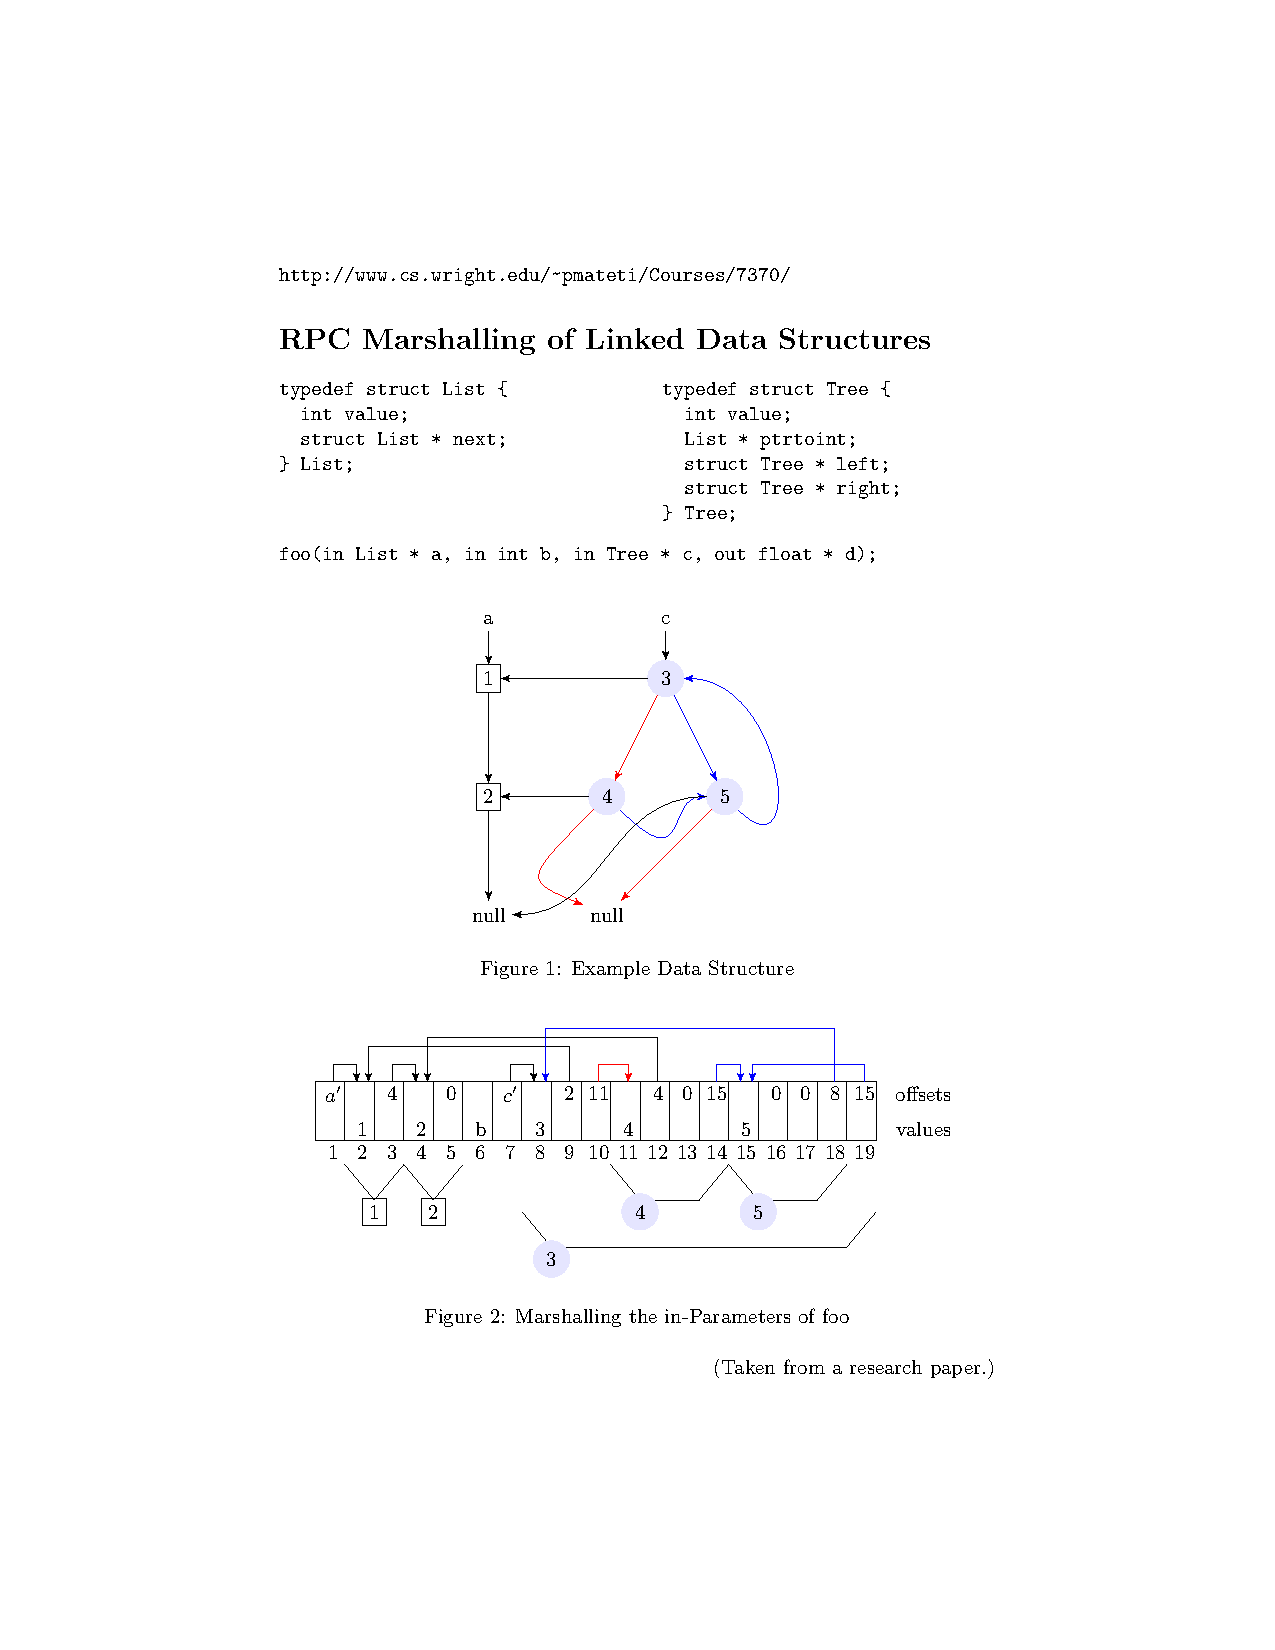
\includegraphics[scale=0.25]{Figures/rpc-marshalling-tikz.pdf}
\end{minipage}
\quad
\quad
\begin{minipage}{5.0cm}
  The left hand figure is produced by {\tt includegraphics \{
    Figures/rpc-marshalling-tikz.pdf \}}.  That is a single page pdf
  with some text and a nicely drawn diagram using TiKZ; click
  \url{./Figures/rpc-marshalling-tikz.pdf} to see it in full size.
\end{minipage}

\subsection{Graphical Plots}

Take your  data, and generate a .png or .pdf file, e.g., using
{\tt gnuplot}.


\section{Tables}

Tables should generally be no more than a single page.  But, if you
must have long tables, look up the packages named {\tt tabularx,
  longtable} and {\tt ltxtable}.

\begin{table}[htb]
\centering
\begin{tabular}{|p{3.75cm}|r|r|r|r|r|}\hline
Category                & {\tt tcpdump} & {\tt sniffit} & {\tt hunt}  &
{\tt dsniff}  & {\tt ethereal} \\ \hline\hline
Word Count & 218455 & 30938   & 45568 & 66599   & 1352372\\ \hline
Lines of Code & 36085  & 3005    & 8817  & 9680    & 280068\\ \hline
Binary Size (Kb) & 488    & 53      & 384   & 482     & 500\\ \hline
Cyclomatic Complexity & 5392   &610      & 2029  & 1517    & na\\ \hline
\end{tabular}


%Actual Binary Size             & 500663 & 54060 & 393700  & 493589  & 3155609 \\ \hline

\caption{Size Summaries of the Selected Sniffers}\label{metric}
\end{table}

\section{Inclusion of Algorithms, ..., Source Code}

Consider ``doing'' literate programming \cite{LP-KNUTH}.

\subsection{Verbatim Mode}

Short pieces of source code can be included in the verbatim mode.  In
this mode, the special characters of \TeX{} are produced as-is.
However, the TAB characters are ignored.  Indentation should therefore
use just blanks.

\begin{verbatim}
#!/bin/bash
# kppp does not correctly set the PPP up.  Here is the fix.
#

fix-ppp() {
    route del -net 0.0.0.0
    route add default gw 130.108.108.8
    route -n
}
\end{verbatim}

For long listings, see \url{en.wikibooks.org/wiki/LaTeX/Source_Code_Listings}.

\subsection{Algorithms}

\newcommand\cupEq{\protect{~\cup{\kern -0.5em}=~}}
\newcommand\plusEq{\protect{~+{\kern -0.5em}=~}}
\newcommand{\OMath}{\ensuremath{\mathcal{O}}}
\renewcommand{\emptyset}{\{\}}
\newcommand\on[2]{{\bf on}{~}{#1}{~\bf do~}{#2}}
\newcommand\bang{{\bf !}~}
\newcommand\query{{\bf ?}~}


\begin{figure}[h]
\begin{minipage}{.45\textwidth}
\begin{algorithm}[H]
  $K_1  := x := 0$\;
  \ForAll {$A \sqsubseteq B \in \OMath_1$} {
    UN \bang update$(B_U, A)$ \query $x$\;
    $K_1 \plusEq x$\;
  }
~\\
  \caption{$A \sqsubseteq B \Rightarrow U[B] \sqsubseteq U[A]$}
  \label{pseudo-R1-2}
\end{algorithm}
\end{minipage}                  % do not insert new lines here
~\textcolor{blue}{\vrule}~
\begin{minipage}{.6\textwidth}
\begin{algorithm}[H]
  $K_2 := x := 0$\;
  \ForAll {$A_1 \sqcap\dots\sqcap A_n\sqsubseteq B \in \OMath_2$} {
    UN \bang $\sqcap(B_U, \{A_1, \dots, A_n\})$ \query $x$\;
    $K_2 \plusEq x$\;
  }
  \label{pseudo-R2-2}
  \caption{{$A_1 \sqcap\dots\sqcap A_n$}
    {$\sqsubseteq B \Rightarrow U[B] \cupEq$}
    {$U[A_1] \cap \dots \cap U[A_n]$}}
\end{algorithm}
\end{minipage}
\caption{Two Algorithms Side-by-Side}
\label{TwoAlgs}
\end{figure}

Figure \ref{TwoAlgs} shows how algorithms can be shown nicely using a
package named {\tt aligorithms2e}; this may need to be installed.  It
created one {\tt figure} using two {\tt minipage}-s.  Several
non-standard math symbols were defined with {\tt newcommand}.
This algorithm is written in pseudo code.

\section{Final v Draft}

The {\tt draft} option is considerably faster than the {\tt final}
when there are many garphical figures.

If you are seeing solid-black rectangles, on some pages, it is because
of the {\tt draft} option in your \verb|\documentclass|.  Change it to
{\tt final}, and these will disappear, but the lines may still stick
out.  Fix these by inserting forced line breaks (usually with
\verb|\\| or \verb|\par|).

% -eof-
